\section{Fast Eagle}
  \subsection{Definición y objetivos}
    \paragraph{El módulo Fast Eagle forma parte de la arquitectura final de Ambienta2MX. El propósito principal de este módulo es brindar la información cartográfica de México por medio de un servicio expuesto, considerando latitud, longitud o nombre de la localidad deseada.}
    \begin{figure}[h!]
        \centering
          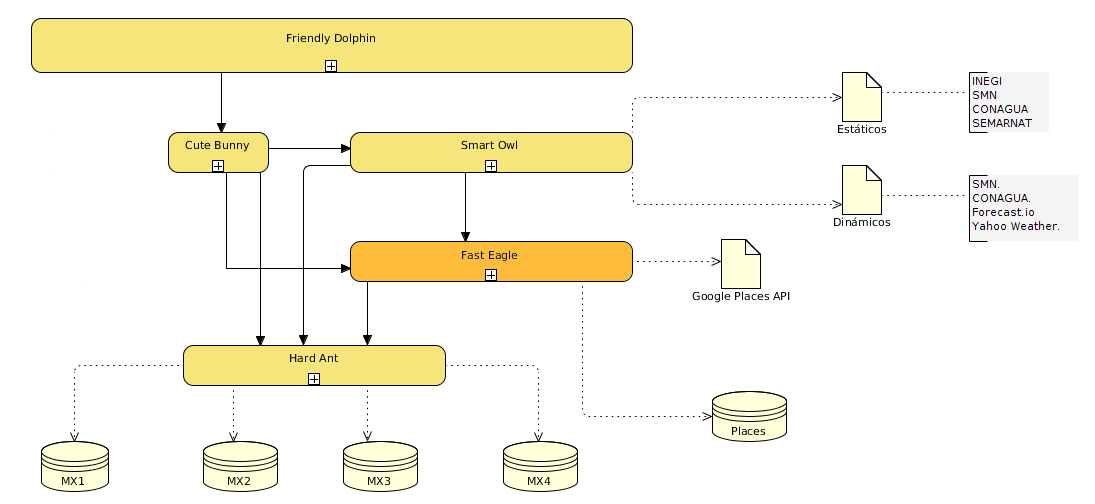
\includegraphics[width=\textwidth]{./images/DiagramaAmbienta2MX_FastEagle.png}
        \caption{Fast Eagle, Módulo de Ambienta2MX.}
    \end{figure}
    \paragraph{Fast Eagle se encargará de exposición de datos brindados por el (Instituto Nacional de Estadística y Geografía) INEGI considerando los su politica de datos públicos que tiene, tomando como base la cartografía del territorio nacional.}
    \paragraph{Actualmente la información que proporciona el INEGI se encuentra en archivos de tipo CSV o bien, terceros se han encargado de estandarizar la información de forma relacional considerando MySQL como gestor principal de información.}
    \paragraph{Sin embargo, por la necesidad de búsquedas geográficas, se generó una migración de la información a un modelo de datos orientado a documentos, siguiendo la especificación GeoJSON en su versión del año 2008. Sólo basta con realizar un proceso de exportación al gestor de de documentos Mongo, y generar los índices geográficos. \cite{35}}
    \paragraph{La información que proporciona el INEGI carece de campos esenciales para la estandarización de la información cartográfica considerando el formato propuesto por el equipo de trabajo, para dar solución a ese contratiempo se hará uso de servicios externos que ya cuentan con información definida, es decir, que su información ha pasado bajo un cierto proceso de limpieza y regulación, por ejemplo, los servicios de Google Places API.}
  \subsection{Alcances}
    \paragraph{Fast Eagle, tendrá como alcance principal el brindar la información de las localidades del territorio nacional utilizando un servicio a demanda, en contraste con otro tipo de recolección como lo es el Crowd Sourcing\cite{37}, las bases dependientes de sistemas externos tendrán siempre una unión, aunque sea mínima,con éstos debido a que la información suele actualizarse de forma periódica.}
    \paragraph{Éste módulo sólo podrá consultar la información utilizando índices georeferenciados y coincidencia parcial con cadenas, es decir, sólo dos tipos de servicios serán expuestos.} 
    \paragraph{Sin embargo, la unión con estos sitemas tiende a ser mínima conforme la comunidad conmienza a hacer uso del módulo o sistema en cuestión.}
  \subsection{Restricciones}
    \paragraph{Una de las principales limitantes del ḿodulo es la dependencia de terceros conforme el proyecto comienze a obtener información, es decir, al ser utilizado como una base a demanda, la información siempre tendrá que ser procesada por un tercero, posteriormente ĺa dependencia será menor conforme los puntos sean más en la base de datos de tipo Places.}
    \paragraph{Al considerar una base orientada a documentos, cómo lo es Mongo, el problema principal es la gestión de la inforación y la posible compatibilidad con otros sistemas, por ejempo, el Stack Geográfico conocido como OSGeo\cite{38}, no soporta consultas de forma directa con este tipo de bases.}
  \subsection{Arquitectura}
    \paragraph{A continuación se muestra con más detalle la arquitectura y diagramas que componen al módulo Fast Eagle. }
    \begin{figure}[h!]
        \centering
          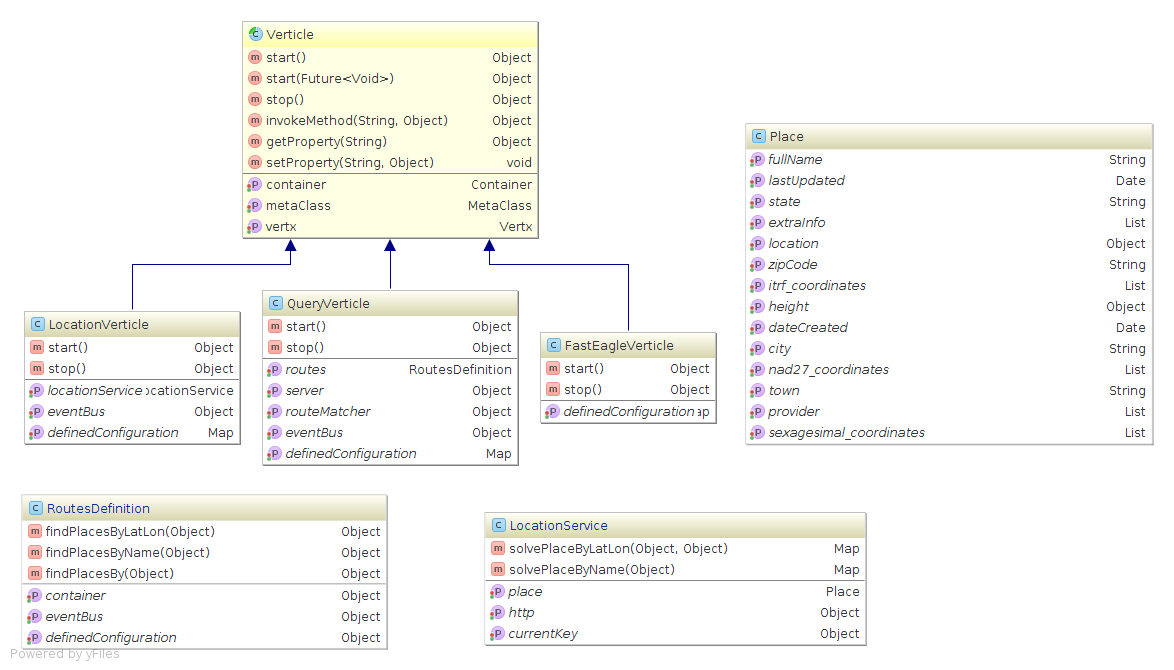
\includegraphics[width=\textwidth]{./images/FastEagleClassDiagram.png}
    \end{figure}
    \paragraph{El objetivo principal de este módulo es brindar a los demás componentes del sistema información cartográfica de una localidad de país, considerando como valores de entrada, latitud y longitud o bien el nombre del lugar.}
    \paragraph{En caso de que no exista la información deseada por el usuario o algún otro módulo del sistema en la cartografía (base de datos llamada Places), Fast Eagle tratará de resolver la información en fuentes externas, persistiendo el modelo resuelto y regresando esa información al solicitante.}
    \begin{figure}[h!]
        \centering
          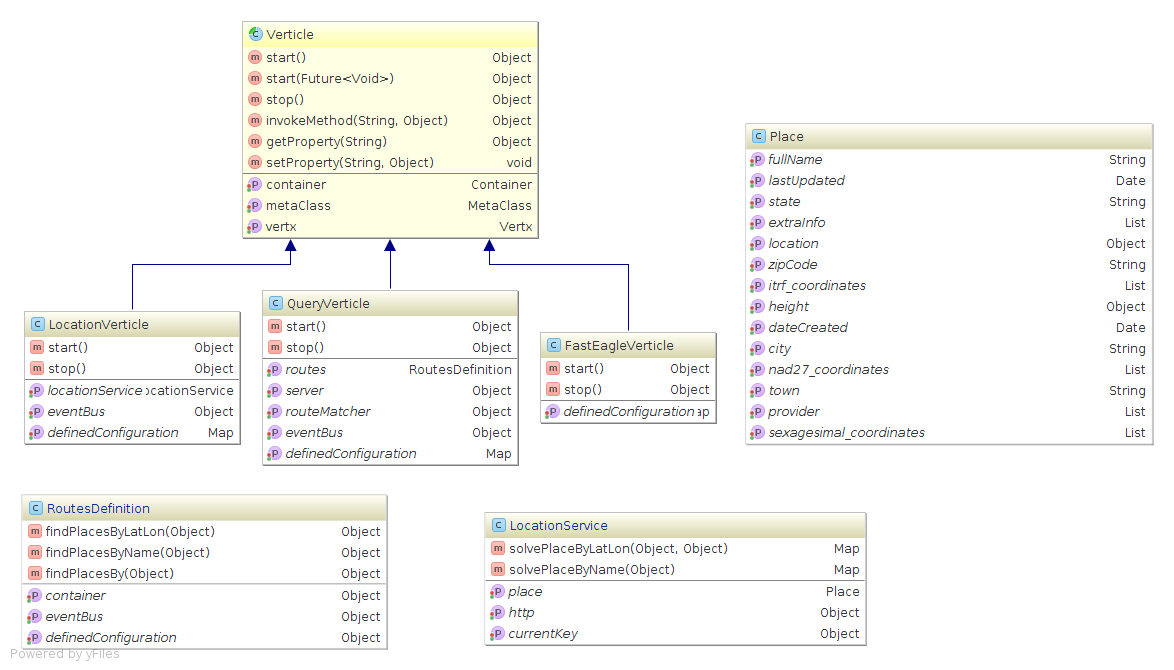
\includegraphics[width=\textwidth]{./images/FastEagleClassDiagram}
    \end{figure}
    \begin{figure}[h!]
        \centering
          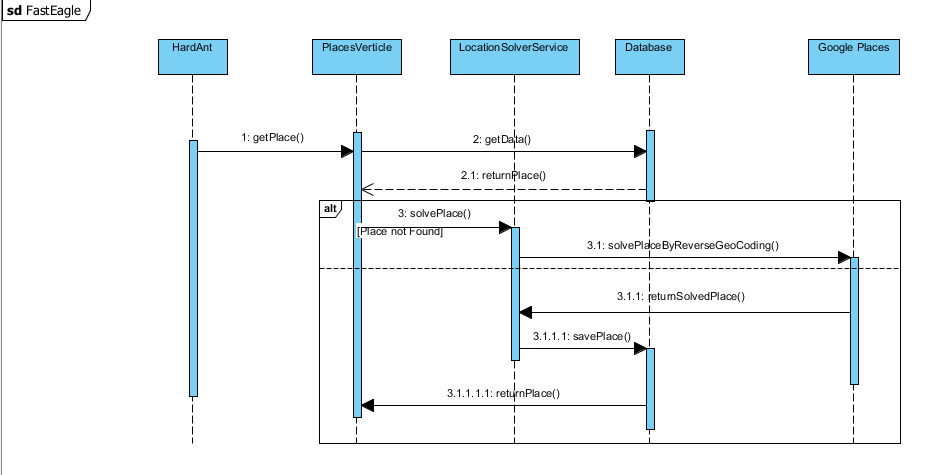
\includegraphics[width=\textwidth]{./images/FastEagleSequenceDiagram}
    \end{figure}
    \paragraph{Fast Eagle cuenta con varios procesos desarrollados, la integración de cada proceso y su respectiva integración da solución a un problema de estandarización, resolución y consulta de datos geográficos vía Latitud, Longitud y Ubicación.}
    \newpage
      \begin{landscape}
        \begin{figure}[b!]
        \centering
        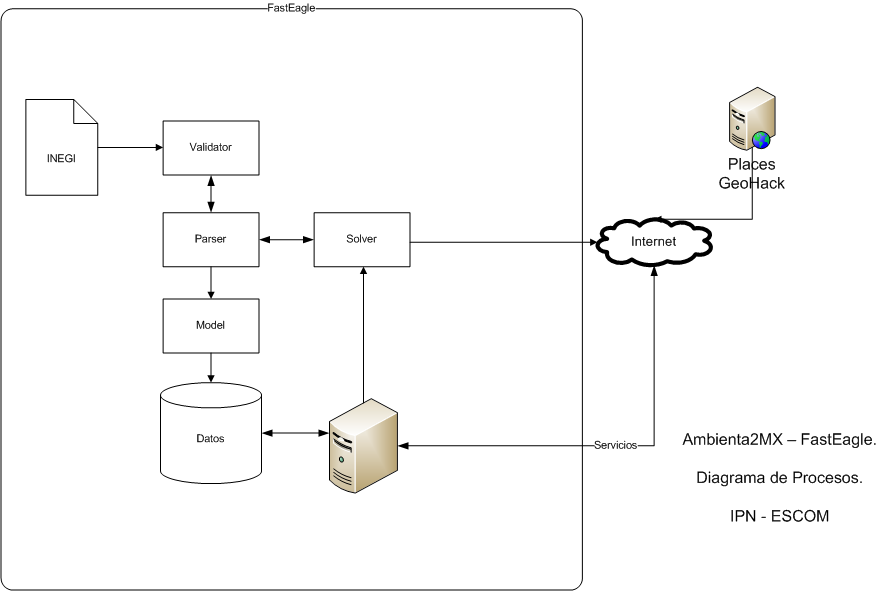
\includegraphics[width=22.5cm,height=12cm]{./images/DiagramaFastEagle}
        \caption{Diagrama por bloques de Fast Eagle}
      \end{figure}
      \end{landscape}
    \newpage
    \paragraph{En el diagrama se muestran tres módulos básicos, estos forman parte del núcleo de Fast Eagle, también podemos observar que se cuenta con la interacción de servicios de terceros como Google Places,  también se cuenta con la exposición de los servicios a través de un servidor web.}
    \paragraph{\textbf{\emph{Parser}} tomará los datos que el proceso de validación le arroje para transformar al estado propuesto por el equipo de trabajo (Véase modelo de datos). Considerando un proceso de resolución en caso de que la información proporcionada por el INEGI se encuentre incompleta no sea válida.}
    \paragraph{Para toda la información que carezca de datos correctos \textbf{\emph{Solver}} buscará una resolución en servicios de terceros, después de la resolución, los datos serán guardados en el gestor de bases de datos bajo el formato propuesto por el equipo de trabajo.}
    \paragraph{\textbf{\emph{Model}} es la capa de interacción con la base de datos, ésta se encarga de las operaciones mejor conocidas como CRUD (Create, Read, Update and Delete),  persistiendo la información en MongoDB, utilizando los canales de Vert.x para su convivencia con la antes mencionada.}
    \paragraph{Para poder exponer los datos, se hará uso de un servidor web minimalista orientado a micro servicios desarrollado en Vert.x, éste será un servicio público que formará parte de la infraestructura final de Ambienta2MX.}
    \paragraph{El servicio expuesto se encargará de las búsquedas a nivel base de datos y en caso de no encontrar la información buscará en terceros para poder agregarla a la base de datos y así ir mejorando el contenido de nuestro índice cartográfico.}
    \paragraph{Considerando las bondades que nos brinda el framework Vert.x, se generó un canal para la resolución de la información utilizando el servicio de Google Maps, éste canal interactúa de forma directa con el servicio de places expuesto a todos los usuarios o módulos del sistema.}
    \paragraph{La comunicació principal será de tipo REST, para el proceso de 
    obtención de información relacionada al territorio nacional.}
  \subsection{Factibilidad}      
    \paragraph{El desarrollo del proyecto se fue orillando a la eliminiación de ciertos procesos ya adecuación de tecnologías. Por ejemplo, la lectura de los archivos del INEGI (Fuentes expuestas en formato CSV), fue reemplazada por el uso de un script de migración entre un gestor público de tipo MySQL hacia un servicio Mongo, realizando también la generación de los índices geográficos.}
    \paragraph{Un problema importante fue la determinación de la cantidad de Verticles (Compomente de Vert.x) por qué un exceso de elementos a desplegar se veía reflejado en la saturación del servicio de base de datos Mongo, esto fue determinado desplegando 20, y posteriormente disminuir el valor hasta llegar al valor de 4.}
  \subsection{Implementación}
    \paragraph{El código y el proyecto como tal se encuentran en línea utilizando Git\cite{38} en conjunto con Github\cite{39}, para el proceso de control de versiones. Para la gestión de tareas y desarrollo del proyecto fue utilizado Gradle en conjunton con Vert.x.}
    \paragraph{Las ventajas que nos ofrece Git/Github es la integración con procesos de desarrollo utilizando metodologías ágiles. La siguiente imagen muestra el control y manejo de issues (análogos a objetivos o features) que fueron desarrollados para cumplir con los objetivos y mejoras planteadas para cada módulo.}
    \begin{figure}[h!]
        \centering
          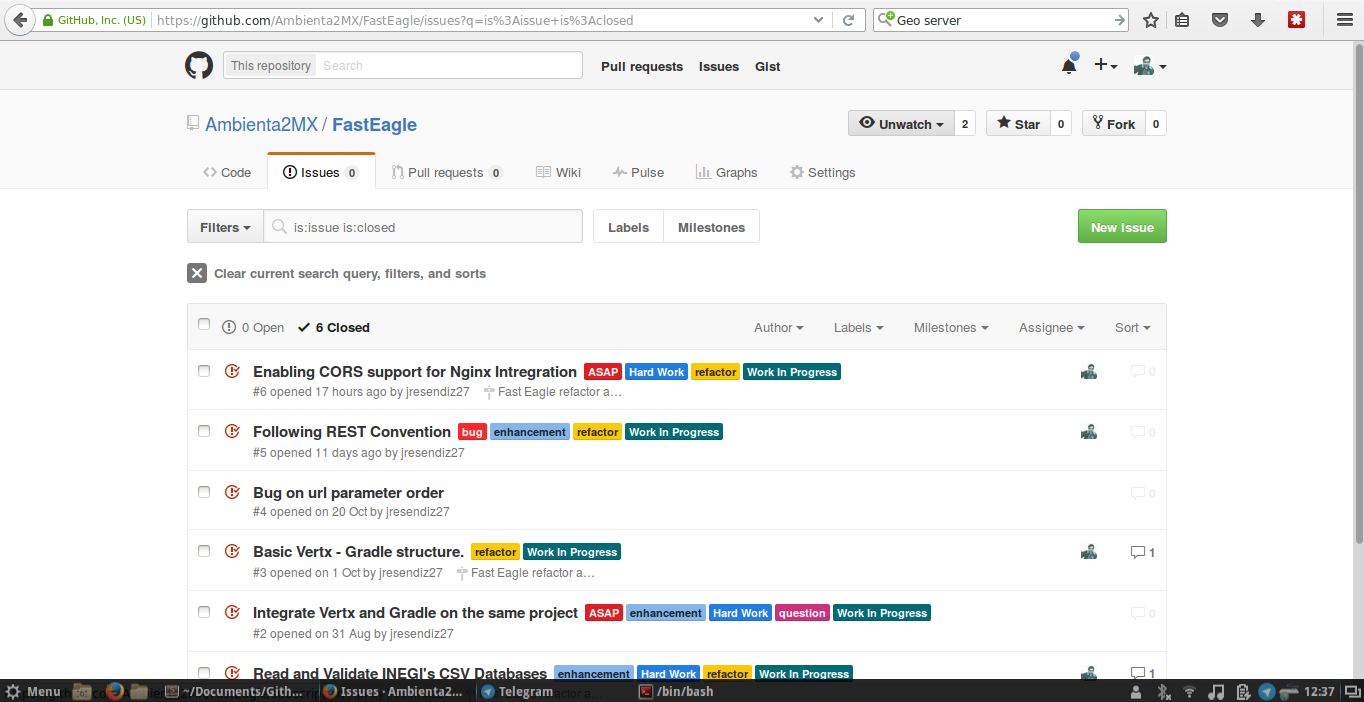
\includegraphics[width=\textwidth]{./images/FastEagleIssues.png}
          \caption{Fast Eagle, Integración con Github.}
    \end{figure}
  \subsection{Pruebas y Capturas de pantalla}
    \paragraph{A continuación se muestran algunas pruebas realizadas y las capturas de pantalla del servicio REST y la respuesta qué este nos regresa.}
    \begin{figure}[h!]
      \centering
        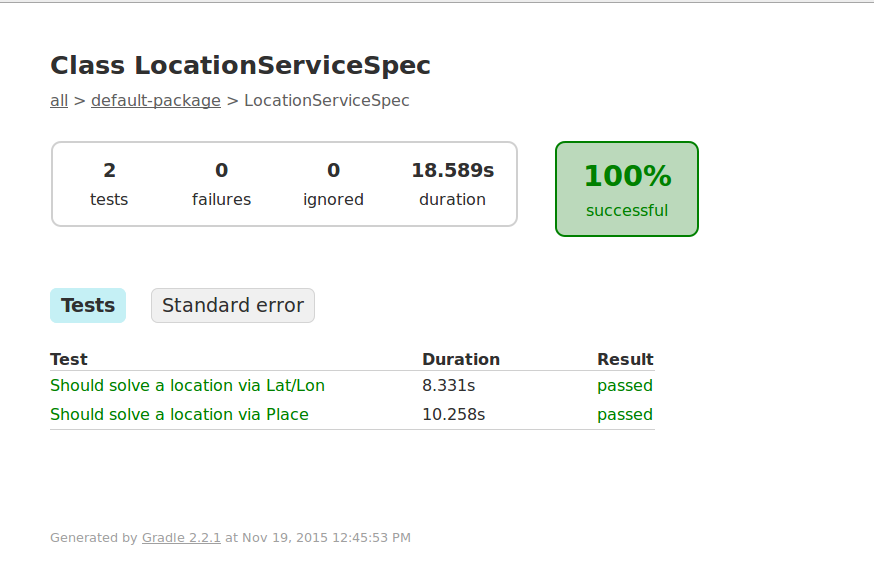
\includegraphics[width=\textwidth]{./images/PruebasFastEagle}
        \caption{Fast Eagle, Pruebas de Fast Eagle.}
    \end{figure}
    \begin{figure}[h!]
      \centering
        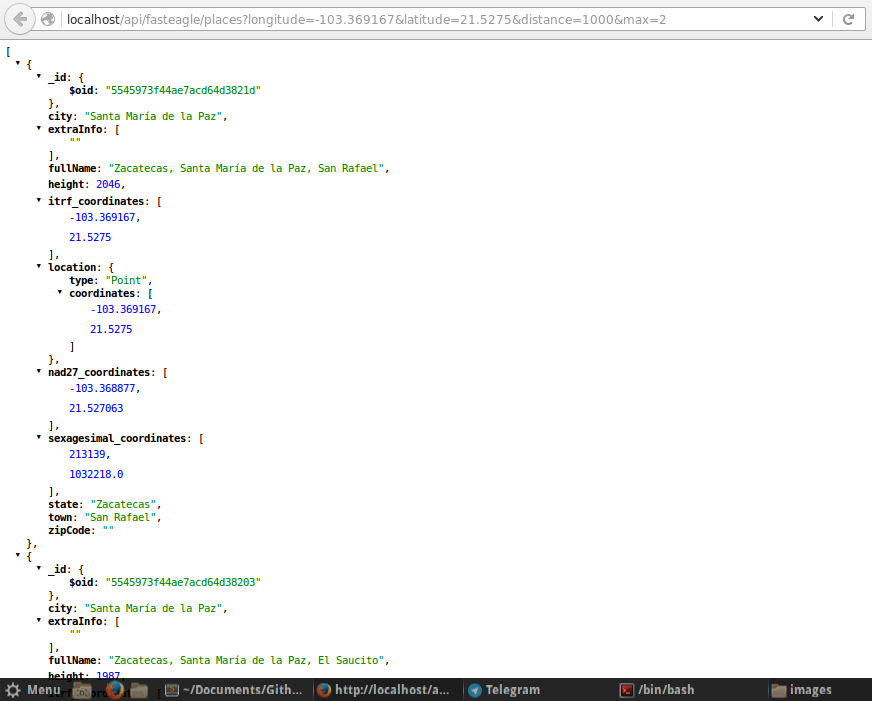
\includegraphics[width=\textwidth]{./images/CapturaFastEagle}
        \caption{Fast Eagle, Respuesta del servicio rest.}
    \end{figure}